\documentclass[11pt]{beamer}
\usepackage[OT1]{fontenc}
\usepackage[utf8x]{inputenc}
\usepackage[frenchb]{babel}
%\usepackage[dvipsnames]{xcolor}
\usepackage{xcolor}
\usetheme{Cpr}
\title{\textbf{Cahier des charges}}
\subtitle{Communication et conception d'un projet de recherche et/ou développement}
\date{5 Décembre 2012}
\author{Arnaud \textsc{Frèche} \\ Charlotte \textsc{Héricé} \\ Sarai \textsc{Mola}\\ Typhaine  \textsc{Paysan-Lafosse} \\ Joris \textsc{Sansen}}
\institute[Université Bordeaux 1] {Master 2 BioInformatique}
\setbeamertemplate{navigation symbols}{}
\begin{document}

\frame{\titlepage}

%\section*{Sommaire}

%\begin{frame}
 % \tableofcontents
%\end{frame}

%%%%%%%%%%%%%%%%%%%%%%%%%%%%%%%%%%
\section{Introduction}			
%%%%%%%%%%%%%%%%%%%%%%%%%%%%%%%%%%

\begin{frame}
	\frametitle{\secname}
	\begin{minipage}{6cm}
	Réseaux Métaboliques
	\begin{figure}[h]
		\begin{center}
   			\begin{minipage}[c]{0.9\textwidth}
  				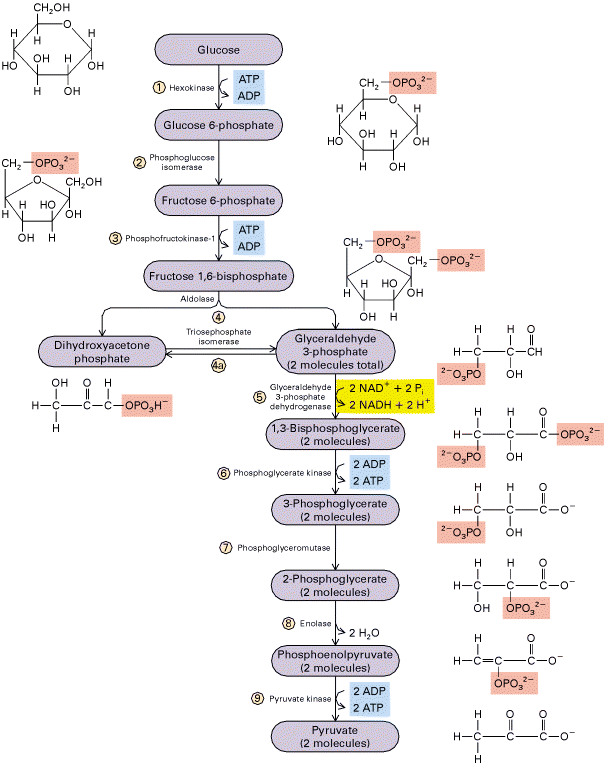
\includegraphics[scale=0.2]{glycolyse.png}
			 \end{minipage}
  		\end{center}	
	\end{figure}
	\end{minipage}
	\begin{minipage}{4cm}
   		Modes Élémentaires
   		\newline

		\begin{figure}[h]
			\begin{center}
   				\begin{minipage}[c]{0.9\textwidth}
  					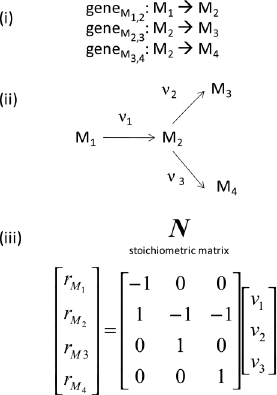
\includegraphics[scale=3]{modelem.png}
				 \end{minipage}
  			\end{center}	
		 \end{figure}
	\end{minipage}
\end{frame}

%%%%%%%%%%%%%%%%%%%%%%%%%%%%%%%%%%
\section{Contexte}			
%%%%%%%%%%%%%%%%%%%%%%%%%%%%%%%%%%

\begin{frame}
	\frametitle{\secname}
	\begin{minipage}{5cm}
	\begin{block}{Sujet}
		\begin{itemize}
		\item Calcul de flux
		\item \textit{regEfmtool}
		\end{itemize}
	\end{block}
	\begin{block}{Objectifs}
		\begin{itemize}
		\item Interface Graphique
		\item Technologies Web
		\end{itemize}
	\end{block}
	\end{minipage}
	\begin{minipage}{5cm}
	\begin{figure}[h]
			\begin{center}
			%\fbox{
   				\begin{minipage}[c]{0.9\textwidth}
  					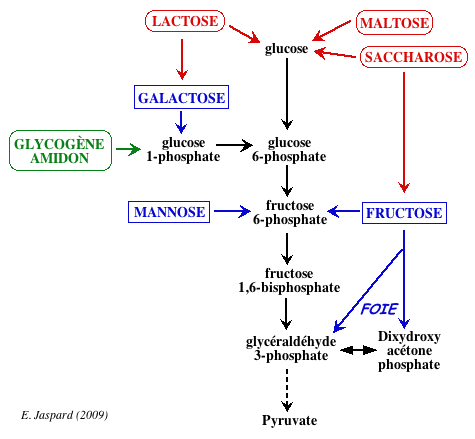
\includegraphics[scale=0.3]{pyruvate.png}
				 \end{minipage}%}
  			\end{center}	
		 \end{figure}
	\end{minipage}
\end{frame}

%%%%%%%%%%%%%%%%%%%%%%%%%%%%%%%%%%
\section{État de l'existant}			
%%%%%%%%%%%%%%%%%%%%%%%%%%%%%%%%%%

\begin{frame}
	\frametitle{\secname}
	\begin{minipage}{5cm}
	\begin{block}{CellNetAnalyser}
	\begin{itemize}
	\item Package de MATLAB
	\item Analyse fonctionnelle et structurelle de résaux biochimiques
	\item Calcul des modes élémentaires grâce à METATOOL
	\end{itemize}
	\end{block}
	\end{minipage}
	\begin{minipage}{5cm}
	\begin{center}
	\begin{figure}[h]
	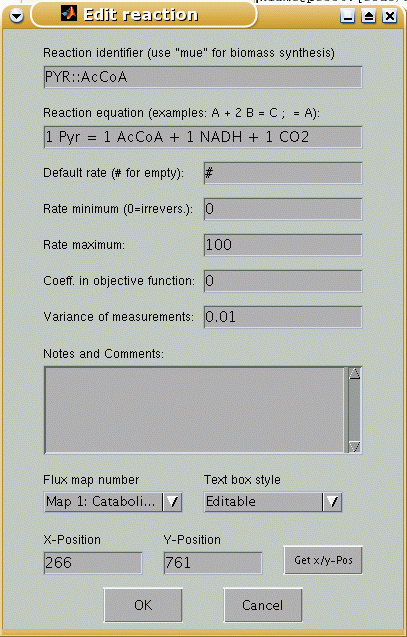
\includegraphics[scale=0.3]{cellnet.png}
		
	\end{figure}
	\end{center}
	\end{minipage}
		
\end{frame}

\begin{frame}
\frametitle{\secname}
	\begin{block}{MetaTool}
	\begin{itemize}
	\item Étude structure réseaux métaboliques
	\item Calcul des modes élémentaires
	\item Module de MATLAB 
	\item Format entrée: fichier \textit{.dat}, format sortie: fichier \textit{.out}
	
	\end{itemize}
	\end{block}	
	
	\begin{block}{RegEfmtool}
	\begin{itemize}
	\item Extension d'\textit{Efmtool}
	\item Calcul des modes élementaires de flux
	\item Régulation transcriptionnelle du réseau métabolique
	\item Fichiers textes formatés en entrée
	\end{itemize}
	\end{block}
\end{frame}

%%%%%%%%%%%%%%%%%%%%%%%%%%%%%%%%%%
\section{Besoins	}	
%%%%%%%%%%%%%%%%%%%%%%%%%%%%%%%%%%

\subsection{Besoins fonctionnels}

\begin{frame}
	\frametitle{\subsecname}
	\begin{block}{Besoins fonctionnels}
		\begin{itemize}
		\item Interface Homme-Machine
		\item Chargement des données
		\item Réglage des paramètres et aide utilisateur
		\item Résultats
		\end{itemize}
	\end{block}
\end{frame}

\subsection{Maquette}

\begin{frame}
	\frametitle{\subsecname}
	\begin{figure}[h]
		\begin{center}
		\fbox{
   			\begin{minipage}[c]{0.9\textwidth}
  				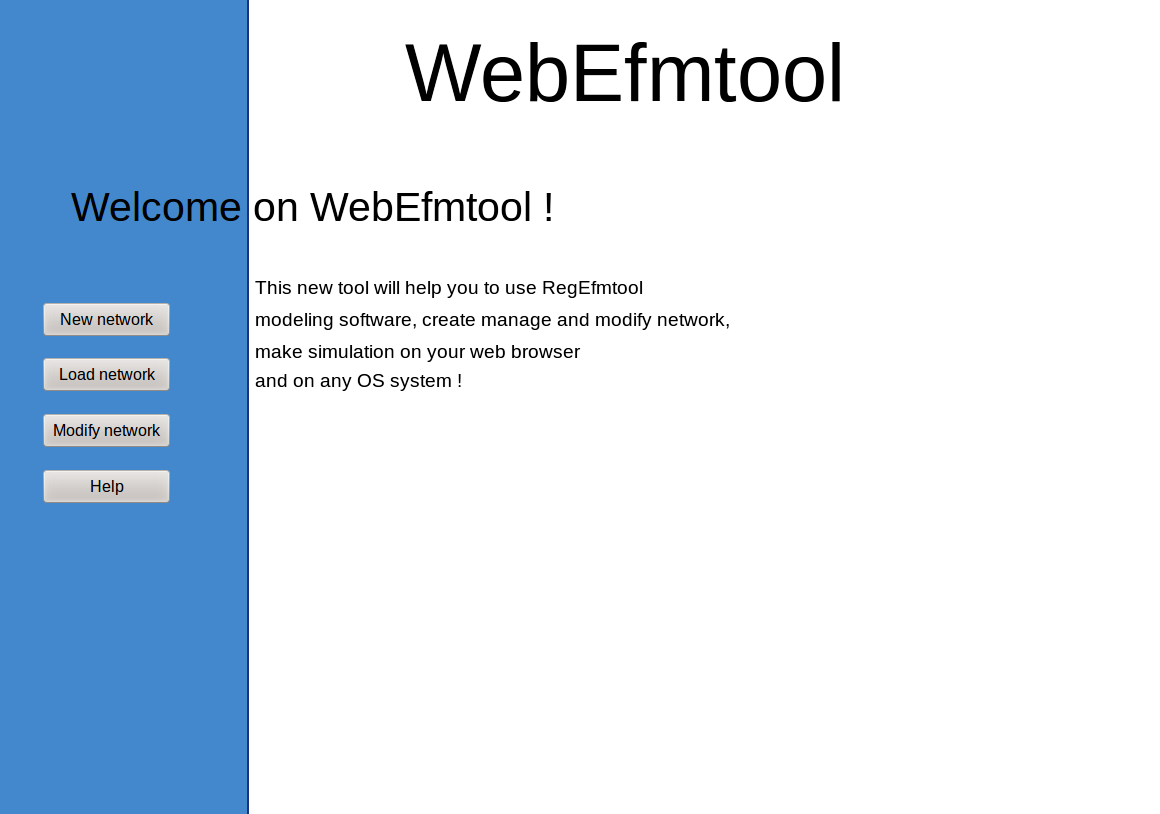
\includegraphics[scale=0.25]{Accueil.png}
			 \end{minipage}}
  		\end{center}	
	 \end{figure}
\end{frame}

\begin{frame}
	\frametitle{\subsecname}
	\begin{figure}[h]
		\begin{center}
		\fbox{
   			\begin{minipage}[c]{0.9\textwidth}
  				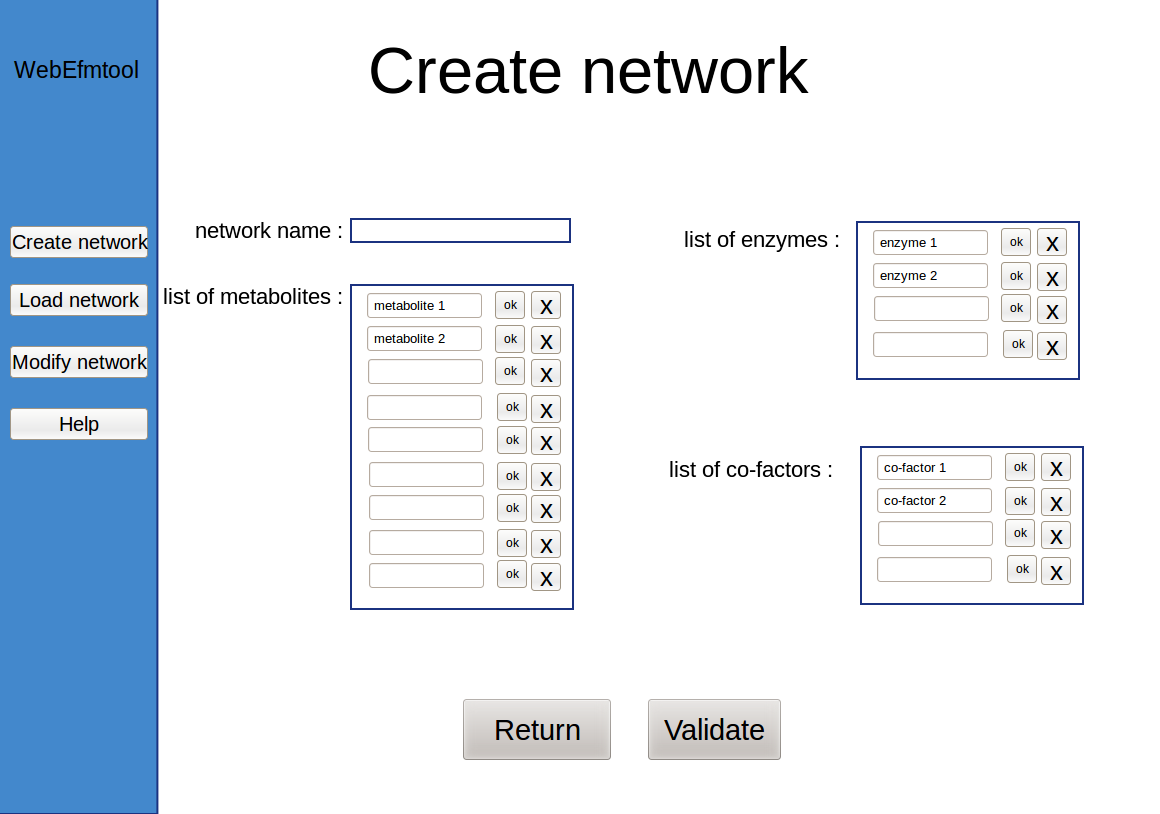
\includegraphics[scale=0.25]{CreateNetwork.png}
			 \end{minipage}}
  		\end{center}	
	 \end{figure}
\end{frame}

\begin{frame}
	\frametitle{\subsecname}
	\begin{figure}[h]
		\begin{center}
		\fbox{
   			\begin{minipage}[c]{0.9\textwidth}
  				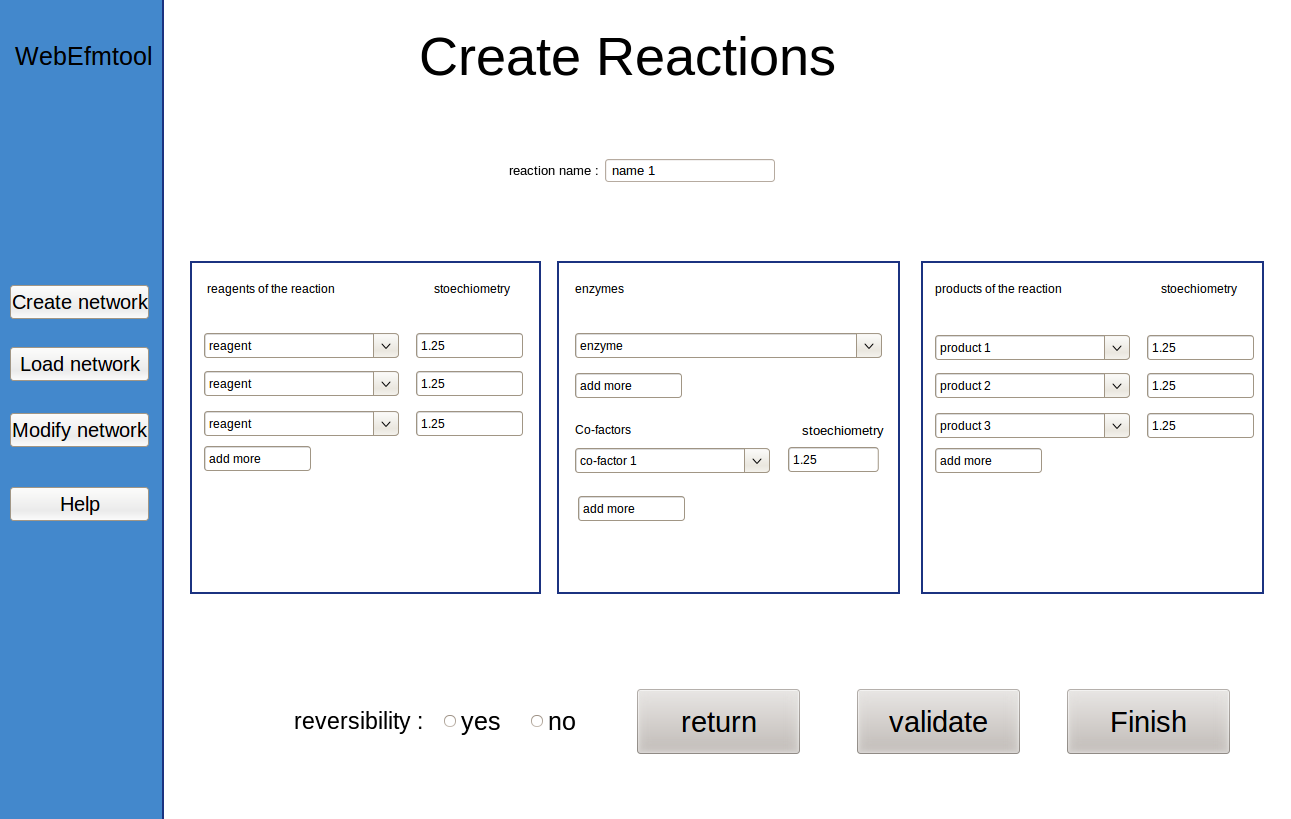
\includegraphics[scale=0.20]{CreateReac.png}
			 \end{minipage}}
  		\end{center}	
	 \end{figure}
\end{frame}

\begin{frame}
	\frametitle{\subsecname}
	\begin{figure}[h]
		\begin{center}
		\fbox{
   			\begin{minipage}[c]{0.9\textwidth}
  				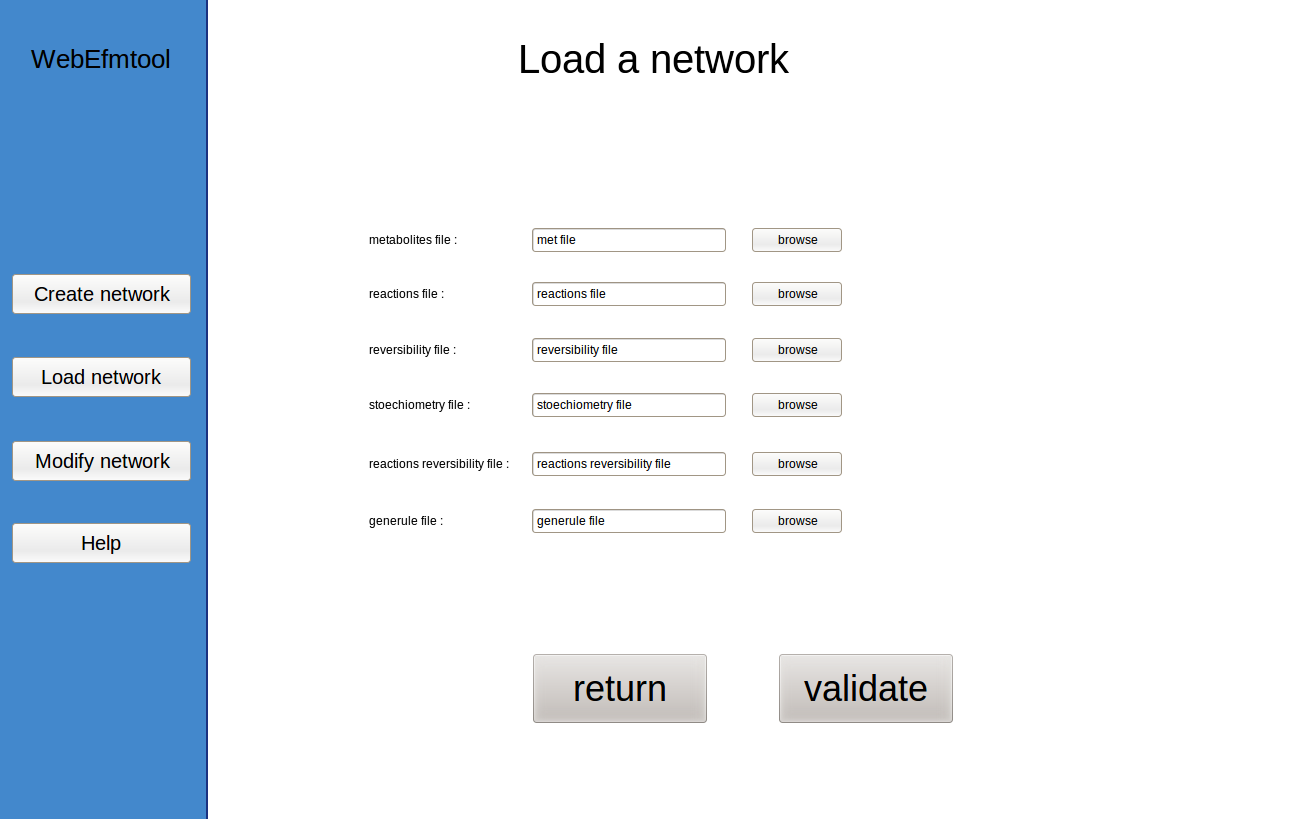
\includegraphics[scale=0.25]{Load.png}
			 \end{minipage}}
  		\end{center}	
	 \end{figure}
\end{frame}

\begin{frame}
	\frametitle{\subsecname}
	\begin{figure}[h]
		\begin{center}
		\fbox{
   			\begin{minipage}[c]{0.9\textwidth}
  				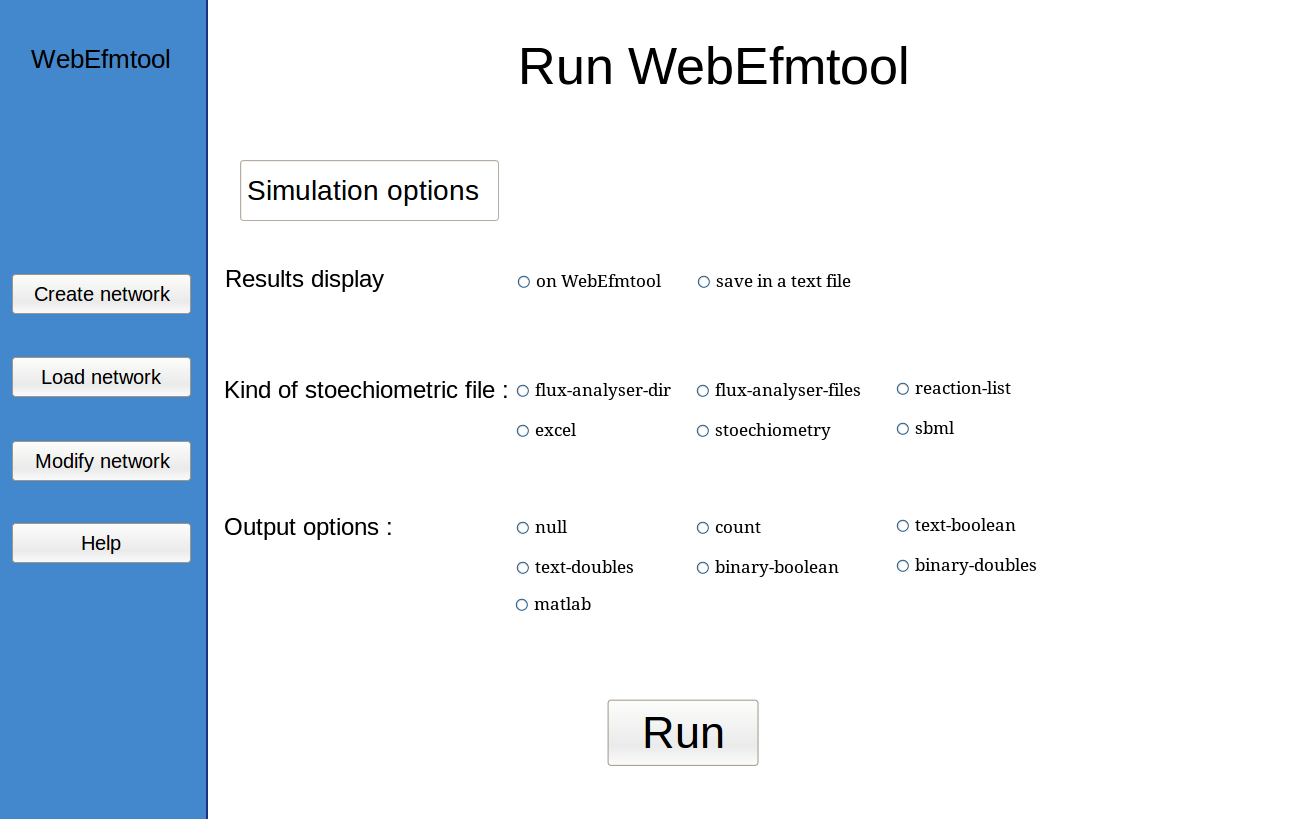
\includegraphics[scale=0.25]{Run.png}
			 \end{minipage}}
  		\end{center}	
	 \end{figure}
\end{frame}

\begin{frame}
	\frametitle{\subsecname}
	\begin{figure}[h]
		\begin{center}
		\fbox{
   			\begin{minipage}[c]{0.9\textwidth}
  				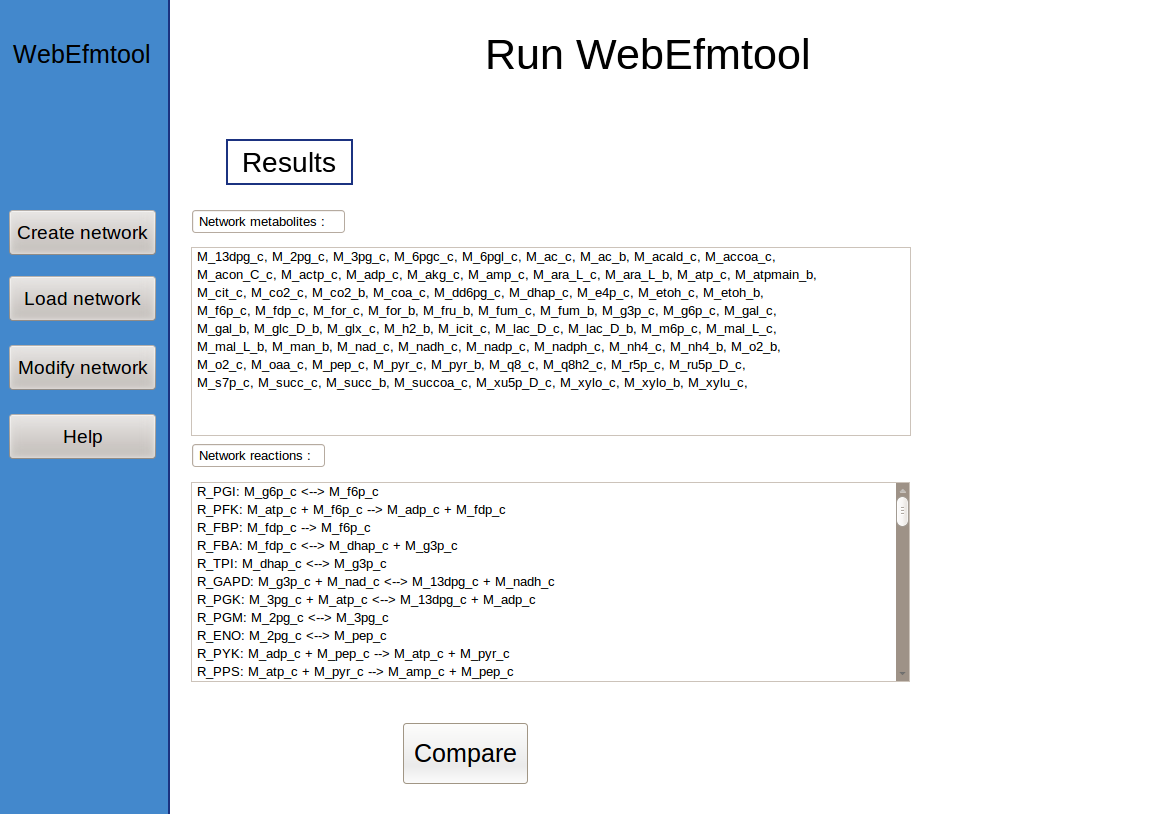
\includegraphics[scale=0.25]{result_view.png}
			 \end{minipage}}
  		\end{center}	
	 \end{figure}
\end{frame}

\begin{frame}
	\frametitle{\subsecname}
	\begin{figure}[h]
		\begin{center}
		\fbox{
   			\begin{minipage}[c]{0.9\textwidth}
  				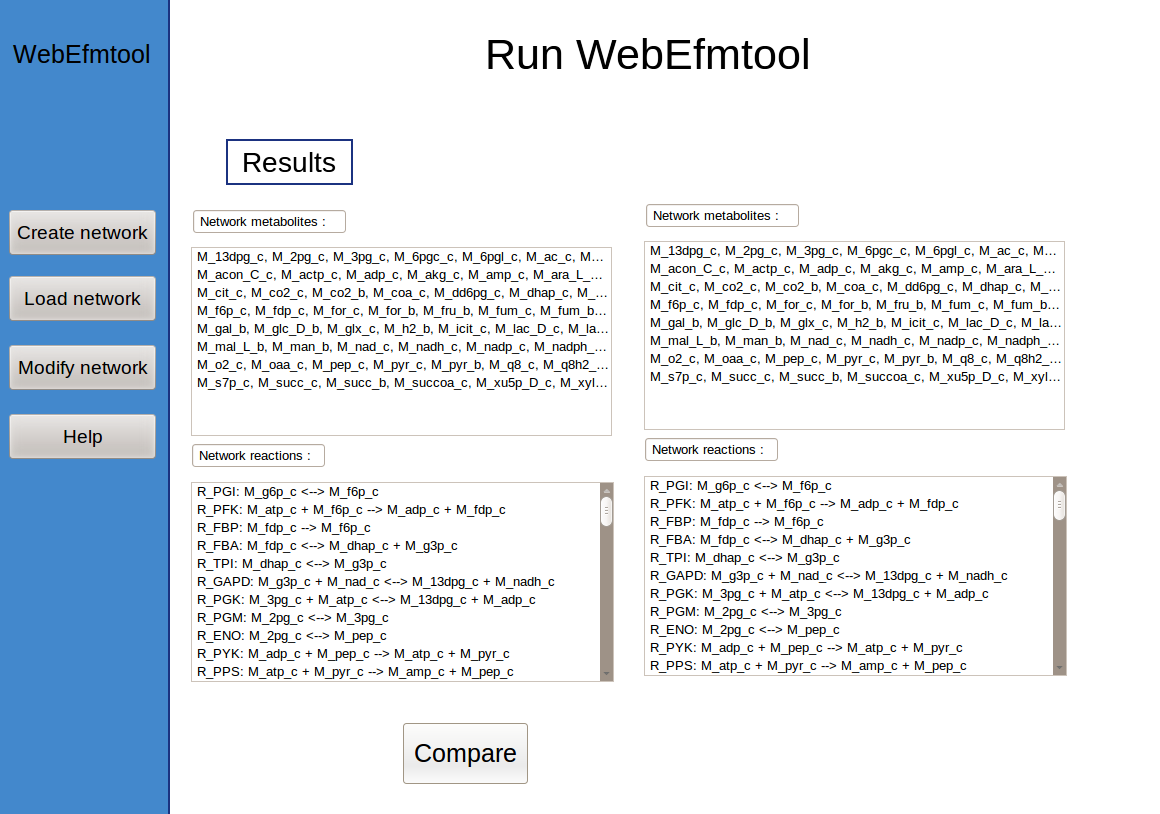
\includegraphics[scale=0.25]{result_compare.png}
			 \end{minipage}}
  		\end{center}	
	 \end{figure}
\end{frame}

\subsection{Besoins non fonctionnels}

\begin{frame}
	\frametitle{\subsecname}
	\begin{block}{Besoins non fonctionnels}
		\begin{itemize}
		\item Portabilité
		\item Sécurité et robustesse
		\item Temps de calcul
		\item Documentation
		\end{itemize}
	\end{block}
\end{frame}

%%%%%%%%%%%%%%%%%%%%%%%%%%%%%%%%%%
\section{Choix et justifications	}	
%%%%%%%%%%%%%%%%%%%%%%%%%%%%%%%%%%

\begin{frame}
	\frametitle{\secname}
	\begin{block}{Langages}
		\begin{itemize}
		\item Structure (squelette du site) = HTML
\item Design = CSS
\item Animation, interactivité = Javascript
\item Communication avec Base de données = PHP

		%\item Base de données 
		\end{itemize}
	\end{block}
\end{frame}

\begin{frame}
	\frametitle{\secname}
	\begin{block}{Accessibilité}
	\begin{itemize}
	\item Différents niveaux d'utilisation possibles: basique ou avancé
	\item Séparation de la partie graphique et de la partie calculs
	\item Documentation
	\end{itemize}
	\end{block}
\end{frame}

\end{document}